\documentclass{article}
\usepackage{graphicx}
\usepackage{amsmath}
\usepackage{amssymb}
\usepackage{amsfonts}
\usepackage{graphicx}

\title{MEMAD-T02}
\author{ALEJANDRO ZARATE MACIAS}
\date{1 de Septiembre 2025}

\begin{document}

\maketitle

% ========================================
% INTRODUCCIÓN
% ========================================
\section*{Introducción}

Para la tarea de esta semana se busca trabajar problemas de optimización de funciones, búsqueda de puntos críticos y su clasificación como máximos o mínimos. Además de probar ciertas propiedades como lo son las matrices definidas positivas o negativas.
La idea es utilizar lo aprendido en los videos proporcionados como material de estudio, así como los libros sugeridos para el curso. Todo esto con el fin de aplicar:
\begin{itemize}
    \item Búsqueda y clasificación de puntos críticos
    \item Análisis de matrices Hessianas
    \item Matrices definidas positivas y negativas
    \item Métodos de optimización
\end{itemize}

% ========================================
% SECCIÓN 1
% ========================================
\section{Problema 1}

\subsection{Enunciado}
Para cada una de las siguientes funciones, encuentre los valores máximo y mínimo en los intervalos indicados, hallando los puntos del intervalo donde la derivada es $0$ y comparando los valores en esos puntos con los valores en los extremos.

\begin{enumerate}
  \item[(a)] $f(x) = x^{3} - x^{2} - 8x + 1$ en $[-2,\,2]$
  \item[(b)] $f(x) = \dfrac{x}{x^{2}-1}$ en $[0,\,5]$
\end{enumerate}

\subsection{Metodología}

Para encontrar los valores máximo y mínimo de una función en un intervalo cerrado, seguimos estos pasos:
\begin{enumerate}
    \item Calcular la primera derivada de la función.
    \item Encontrar los puntos críticos resolviendo $f'(x) = 0$.
    \item Verificar que los puntos críticos estén dentro del intervalo dado.
    \item Clasificar los puntos críticos usando la segunda derivada.
    \item Evaluar la función en los puntos críticos y en los extremos del intervalo.
\end{enumerate}

\subsection{Resultados}
\setcounter{equation}{0}

\textbf{Inciso (a): $f(x) = x^{3} - x^{2} - 8x + 1$ en $[-2,\,2]$}

Primero calculamos la derivada:
\begin{align}
f'(x) &= 3x^{2} - 2x - 8
\end{align}

Para encontrar los puntos críticos, resolvemos $f'(x) = 0$:
\begin{align}
3x^{2} - 2x - 8 &= 0
\end{align}

Usando la fórmula cuadrática:
\begin{align}
x &= \frac{2 \pm \sqrt{4 + 96}}{6} \\
&= \frac{2 \pm \sqrt{100}}{6} \\
&= \frac{2 \pm 10}{6}
\end{align}

Por lo tanto, tenemos que $x_1$ es:
\begin{align}
x_{1} &= \frac{2 + 10}{6} \\
&= \frac{12}{6} \\
&= 2 \\
\end{align}

Y por otra parte, $x_2$ es:

\begin{align}
    x_{2} &= \frac{2 - 10}{6} \\
    &= \frac{-8}{6} \\
    &= -\frac{4}{3}
\end{align}

Ambos puntos críticos están dentro del intervalo $[-2, 2]$.

Ahora clasificamos los puntos críticos usando el criterio de la segunda derivada:
\begin{align}
f''(x) &= 6x - 2
\end{align}

Para $x_1 = -\frac{4}{3}$:
\begin{align}
f''\left(-\frac{4}{3}\right) &= 6\left(-\frac{4}{3}\right) - 2 \\
&= -8 - 2 \\
&= -10 \\
&10 < 0
\end{align}

Como $f''(-\frac{4}{3}) < 0$, el punto $x = -\frac{4}{3}$ es un máximo local.

Para $x_2 = 2$:
\begin{align}
f''(2) &= 6(2) - 2 \\
&= 12 - 2 \\
&= 10 \\
&10> 0
\end{align}

Como $f''(2) > 0$, el punto $x = 2$ es un mínimo local.

Ahora evaluamos $f(x)$ en los puntos críticos y en los extremos:

En $x = -2$:
\begin{align}
f(-2) &= (-2)^{3} - (-2)^{2} - 8(-2) + 1 \\
&= -8 - 4 + 16 + 1 \\
&= 5
\end{align}

En $x = -\frac{4}{3}$:
\begin{align}
f\left(-\frac{4}{3}\right) &= \left(-\frac{4}{3}\right)^{3} - \left(-\frac{4}{3}\right)^{2} - 8\left(-\frac{4}{3}\right) + 1 \\
&= -\frac{64}{27} - \frac{16}{9} + \frac{32}{3} + 1 \\
&= -\frac{64}{27} - \frac{48}{27} + \frac{288}{27} + \frac{27}{27} \\
&= \frac{-64 - 48 + 288 + 27}{27} \\
&= \frac{203}{27}
\end{align}

En $x = 2$:
\begin{align}
f(2) &= 2^{3} - 2^{2} - 8(2) + 1 \\
&= 8 - 4 - 16 + 1 \\
&= -11
\end{align}


\textbf{Inciso (b): $f(x) = \dfrac{x}{x^{2}-1}$ en $[0,\,5]$}

Calculamos la derivada usando la regla del cociente:
\begin{align}
f'(x) &= \frac{(x^{2}-1)(1) - x(2x)}{(x^{2}-1)^{2}} \\
&= \frac{x^{2} - 1 - 2x^{2}}{(x^{2}-1)^{2}} \\
&= \frac{-x^{2} - 1}{(x^{2}-1)^{2}} \\
&= \frac{-(x^{2} + 1)}{(x^{2}-1)^{2}}
\end{align}

Para encontrar puntos críticos, resolvemos $f'(x) = 0$:
\begin{align}
\frac{-(x^{2} + 1)}{(x^{2}-1)^{2}} &= 0
\end{align}

Esto ocurre cuando el numerador es cero:
\begin{align}
-(x^{2} + 1) &= 0 \\
x^{2} + 1 &= 0 \\
x^{2} &= -1 \\
x &= \sqrt{-1}
\end{align}

Esta ecuación no tiene soluciones reales, por lo que no hay puntos críticos en $\mathbb{R}$.

Evaluamos en los extremos del intervalo:

En $x = 0$:
\begin{align}
f(0) &= \frac{0}{0^{2} - 1} = \frac{0}{-1} = 0
\end{align}

En $x = 5$:
\begin{align}
f(5) &= \frac{5}{5^{2} - 1} = \frac{5}{25 - 1} = \frac{5}{24}
\end{align}

\subsection{Discusión}

\textbf{Inciso (a):} 
Comparando los valores obtenidos:
- $f(-2) = 5$
- $f(-4/3) = 203/27 \approx 7.52$  
- $f(2) = -11$

El valor máximo es $203/27$ en $x = -4/3$ y el valor mínimo es $-11$ en $x = 2$.

\textbf{Inciso (b):}
Como no hay puntos críticos en el intervalo, solo comparamos los extremos:
- $f(0) = 0$
- $f(5) = 5/24 \approx 0.21$

El valor máximo es $5/24$ en $x = 5$ y el valor mínimo es $0$ en $x = 0$.

\subsection{Conclusión}

Para funciones continuas en intervalos cerrados, siempre existen valores máximo y mínimo absolutos. Estos pueden ocurrir en puntos críticos del interior del intervalo o en los extremos. Es esencial evaluar la función en todos los candidatos para determinar los valores extremos correctos.


% ========================================
% SECCIÓN 2
% ========================================
\section{Problema 2}

\subsection{Enunciado}
Si $a_{1} < a_{2} < \cdots < a_{n}$, encuentre el valor mínimo de
\[
f(x) \;=\; \sum_{i=1}^{n} (x - a_i)^2
\]

\subsection{Metodología}

Para encontrar el mínimo de esta función expresada como la sumatoria de cuadrados de $x-a_i$, debemos seguir los siguientes pasos:
\begin{enumerate}
    \item Calcular la primera derivada de la función que aplique para todo $i$.
    \item Igualar la derivada a cero para encontrar puntos críticos.
    \item Verificar que el punto encontrado es un mínimo usando la segunda derivada.
\end{enumerate}

\subsection{Resultados}
\setcounter{equation}{0}

Para encontrar el valor mínimo de $f(x) = \sum_{i=1}^{n} (x - a_i)^2$, calculamos la derivada:

\begin{align}
    f'(x) &= 2\sum_{i=1}^{n} (x - a_i) \\
    &= 2\sum_{i=1}^{n} x - 2\sum_{i=1}^{n} a_i \\
    &= 2nx - 2\sum_{i=1}^{n} a_i
\end{align}

Para encontrar el punto crítico, igualamos $f'(x) = 0$:
\begin{align}
    2nx - 2\sum_{i=1}^{n} a_i &= 0 \\
    2nx &= 2\sum_{i=1}^{n} a_i \\
    x &= \frac{1}{n}\sum_{i=1}^{n} a_i 
\end{align}

Analizando esto, $x$ es la media de todos los valores de $a$

\begin{align}
    x = \bar{a}
\end{align}

La segunda derivada es:
\begin{align}
f''(x) = 2n > 0
\end{align}

Como $f''(x) > 0$, el punto $x = \bar{a}$ es un mínimo.

El valor mínimo de la función es:
\begin{align}
f(\bar{a}) = \sum_{i=1}^{n} (\bar{a} - a_i)^2
\end{align}

\subsection{Discusión}

El resultado muestra que el punto que minimiza la función es $x = \bar{a} = \frac{1}{n}\sum_{i=1}^{n} a_i$, que corresponde a la media de los valores $a_i$.

La segunda derivada $f''(x) = 2n > 0$ confirma que se trata de un valor mínimo, ya que es una constante positiva para cualquier $n > 0$.

El hecho de que la función contenga un solo valor de $x$ nos permitie factorizar fácilmente la expresión, tratando todos los términos $a_i$ como constantes durante la derivación. Esto simplifica considerablemente el proceso.

\subsection{Conclusión}

La media $\bar{a}$ minimiza la funcion de suma de cuadrados. Este resultado se obtuvo de manera directa mediante cálculo diferencial, aprovechando que la variable $x$ aparece de forma uniforme en todos los términos de la suma, lo que facilita la factorización y simplifica los cálculos.

% ========================================
% SECCIÓN 3
% ========================================
\section{Problema 3}

\subsection{Enunciado}
¿Cuál es la relación entre los puntos críticos de $f$ y los de $f^{2}$?

\subsection{Metodología}

Para encontrar la relación entre los puntos críticos de $f$ y $f^2$, aplicamos los teoremas vistos en el temario de la semana:
\begin{enumerate}
    \item Identificar los puntos críticos de la función original $f$.
    \item Identificar los puntos criticos de $f^{2}$.
    \item Comparar ambos conjuntos de puntos críticos para establecer relaciones.
\end{enumerate}

Al no tener algun ejemplo en especifico, se debe de recurrir al analisis de las formas generales en las que se ven estas funciones.

\subsection{Resultados}
\setcounter{equation}{0}
Sea $g(x) = f(x)^2$. Los puntos críticos de $f$ son aquellos donde $f'(x) = 0$.

Para encontrar los puntos críticos de $g(x) = f(x)^2$, calculamos su derivada:
\begin{align}
g'(x) = 2f(x)f'(x)
\end{align}

Los puntos críticos de $g(x)$ ocurren cuando $g'(x) = 0$:
\begin{align}
g'(x) = 2f(x)f'(x) = 0
\end{align}

Esto sucede cuando:
\begin{align}
f(x) = 0 \quad \text{ó} \quad f'(x) = 0
\end{align}

Por lo tanto, los puntos críticos de $f^2$ incluyen:
\begin{itemize}
    \item Todos los puntos críticos de $f$ (donde $f'(x) = 0$)
    \item También los puntos donde $f(x) = 0$ (los ceros de $f$)
\end{itemize}

\subsection{Discusión}

El análisis muestra que el conjunto de puntos críticos de $f^2$ siempre contiene como subconjunto a los puntos críticos de $f$. Esto se debe a que cuando $f'(x) = 0$, automáticamente se cumple que $g'(x) = 2f(x)f'(x) = 0$.

Sin embargo, $f^2$ puede tener puntos críticos adicionales en los ceros de $f$, donde $f(x) = 0$ pero $f'(x) \neq 0$.

Por lo tanto, para toda función cuadrática podemos encontrar sus puntos críticos, y entre estos estarán incluidos todos los puntos críticos de la función original sin elevar al cuadrado.

\subsection{Conclusión}

Los puntos críticos de $f$ forman un subconjunto de los puntos críticos de $f^2$. La función cuadrática $f^2$ conserva todos los extremos de $f$ y puede agregar nuevos extremos en los ceros de $f$, ampliando así el conjunto de puntos críticos.

% ========================================
% SECCIÓN 4
% ========================================
\section{Problema 4}

\subsection{Enunciado}
Entre todos los cilindros circulares rectos de volumen fijo $V$, encuentre aquel con el área de superficie más pequeña.

\subsection{Metodología}

Para resolver este problema de optimización con restricciones, seguimos estos pasos:
\begin{enumerate}
    \item Identificar las variables: radio $r$ y altura $h$ del cilindro.
    \item Establecer la función objetivo: área de superficie $A = 2\pi r^2 + 2\pi rh$.
    \item Aplicar la restricción de volumen fijo: $V = \pi r^2 h$.
    \item Usar la restricción para eliminar una variable y convertir el problema en optimización sin restricciones.
    \item Aplicar cálculo diferencial para encontrar el mínimo.
    \item Verificar que es un mínimo usando la segunda derivada.
\end{enumerate}

\subsection{Resultados}
\setcounter{equation}{0}

Las fórmulas para un cilindro circular recto son:
\begin{align}
V &= \pi r^2 h \\
A &= 2\pi r^2 + 2\pi rh
\end{align}

De la restricción de volumen fijo $V = \pi r^2 h$, despejamos $h$:
\begin{align}
h = \frac{V}{\pi r^2}
\end{align}

Reemplazamos $h$ en la función del área:
\begin{align}
A &= 2\pi r^2 + 2\pi r \cdot \frac{V}{\pi r^2} \\
&= 2\pi r^2 + \frac{2V}{r}
\end{align}

Definimos $f(r) = A = 2\pi r^2 + \frac{2V}{r}$ como nuestra función a minimizar.

Calculamos la primera derivada:
\begin{align}
f'(r) &= 4\pi r - \frac{2V}{r^2}
\end{align}

Igualamos a cero para encontrar el punto crítico:
\begin{align}
4\pi r - \frac{2V}{r^2} &= 0 \\
4\pi r &= \frac{2V}{r^2} \\
4\pi r^3 &= 2V \\
r^3 &= \frac{V}{2\pi} \\
r &= \sqrt[3]{\frac{V}{2\pi}}
\end{align}

Calculamos la segunda derivada:
\begin{align}
f''(r) = 4\pi + \frac{4V}{r^3}
\end{align}

Evaluamos en el punto crítico:
\begin{align}
f''\left(\sqrt[3]{\frac{V}{2\pi}}\right) &= 4\pi + \frac{4V}{\left(\sqrt[3]{\frac{V}{2\pi}}\right)^3} \\
&= 4\pi + \frac{4V}{\frac{V}{2\pi}} \\
&= 4\pi + 8\pi \\
&= 12\pi > 0
\end{align}

Como $f''(r) > 0$, el punto crítico es un mínimo.

Ahora encontramos $h$ sustituyendo el valor de $r$:
\begin{align}
h &= \frac{V}{\pi r^2} \\
&= \frac{V}{\pi \left(\sqrt[3]{\frac{V}{2\pi}}\right)^2} \\
&= \frac{V}{\pi \cdot \left(\frac{V}{2\pi}\right)^{2/3}} \\
&= \frac{V^{1/3}}{\pi^{1/3}} \cdot \frac{(2\pi)^{2/3}}{V^{2/3}} \\
&= 2^{2/3} \cdot \pi^{-1/3} \cdot V^{1/3} \\
&= 2 \cdot \sqrt[3]{\frac{V}{2\pi}} \\
&= 2r
\end{align}

Por lo tanto, $h = 2r$.

Verificamos sustituyendo estos valores en la función original del área:
\begin{align}
A &= 2\pi r^2 + 2\pi rh \\
&= 2\pi r^2 + 2\pi r(2r) \\
&= 2\pi r^2 + 4\pi r^2 \\
&= 6\pi r^2
\end{align}

Sustituyendo $r = \sqrt[3]{\frac{V}{2\pi}}$:
\begin{align}
A &= 6\pi \left(\sqrt[3]{\frac{V}{2\pi}}\right)^2 \\
\end{align}

Esta es el área mínima de superficie para un cilindro de volumen fijo $V$.

\subsection{Discusión}

El resultado principal es que $h = 2r$, lo que significa que la altura del cilindro óptimo es exactamente el doble de su radio. 

La segunda derivada $f''(r) = 12\pi > 0$ confirma que encontramos un mínimo global. Esto tiene sentido porque al usar la restricción de volumen, convertimos el problema en una función de una sola variable donde solo puede haber un punto crítico.

El proceso de sustitución fue clave: usar la restricción $V = \pi r^2 h$ para expresar $h$ en términos de $r$ nos permitió reducir el problema a optimizar una función de una variable.

\subsection{Conclusión}

El cilindro de área mínima con volumen fijo tiene la relación $h = 2r$. Este resultado se obtuvo aplicando cálculo diferencial después de usar la restricción para reducir el problema a una variable. La geometría óptima es más "alta" que "ancha" en comparación con un cilindro donde $h = r$.

% ========================================
% SECCIÓN 5
% ========================================
\section{Problema 5}

\subsection{Enunciado}
Demuestre que la suma de un número positivo y su recíproco es al menos $2$.

\subsection{Metodología}

Cuando nos referimos al recíproco de $a$, estamos hablando de $\frac{1}{a}$, y en esta demostración se debe de validar si es que $a + \frac{1}{a} \geq 2$. Para esto podemos aplicar ciertas técnicas de álgebra básica para jugar con la expresión.

\subsection{Resultados}
\setcounter{equation}{0}

Sea $a > 0$ un número real positivo. Queremos demostrar que:
\begin{align}
a + \frac{1}{a} \geq 2
\end{align}

Partimos de la desigualdad que queremos probar:
\begin{align}
a + \frac{1}{a} \geq 2
\end{align}

Restamos $2$ de ambos lados:
\begin{align}
a + \frac{1}{a} - 2 \geq 0
\end{align}

Factorizamos la expresión del lado izquierdo:
\begin{align}
a\left(a + \frac{1}{a} - 2\right) &\geq 0 \\
a^2 - 2a + 1 &\geq 0 \\
(a - 1)^2 &\geq 0
\end{align}

El cuadrado de cualquier número real siempre es mayor o igual a cero:
\begin{align}
(a - 1)^2 \geq 0 \quad \forall a \in \mathbb{R}
\end{align}

Por lo tanto, $(a - 1)^2 \geq 0$ para todo $a \in \mathbb{R}$, y en particular para $a > 0$.


\subsection{Discusión}

Al despejar la función para que fuera $\geq 0$ se pudo ver de manera fácil que podíamos transformar esta ecuación en una cuadrática al multiplicarla por $a$, dado un binomio cuadrado, y por lógica sabemos que el cuadrado siempre es $\geq 0$, lo cual concuerda con la expresión que teníamos.

El punto clave es que $(a-1)^2 \geq 0$ siempre es verdadero para cualquier número real $a$, y la igualdad se alcanza únicamente cuando $a = 1$. Esto significa que el valor mínimo de $a + \frac{1}{a}$ es exactamente $2$, y se obtiene cuando $a = 1$.

Esta desigualdad también se conoce como la desigualdad aritmético-geométrica para dos términos, ya que $\frac{a + \frac{1}{a}}{2} \geq \sqrt{a \cdot \frac{1}{a}} = 1$, lo que implica $a + \frac{1}{a} \geq 2$.

\subsection{Conclusión}

Después de esta demostración podemos decir que $a + \frac{1}{a} \geq 2$ para todo número positivo gracias a su transformación en un binomio al cuadrado usando álgebra.

% ========================================
% SECCIÓN 6
% ========================================
\section{Problema 6}

\subsection{Enunciado}
Para cada una de las siguientes funciones, encuentre sus puntos críticos y clasifíquelos. Luego, use Python para crear gráficos de contorno de ellas y verificar sus resultados.

\begin{enumerate}
  \item[(a)] $f(x,y) = \ln(x^{2} + y^{2} + 1)$
  \item[(b)] $f(x,y) = x^{2} + y^{2} - x - y + 1$
  \item[(c)] $f(x,y) = e^{x}\cos(y)$
  \item[(d)] $f(x,y) = (x^{2} + y - 11)^{2} + (x + y^{2} - 7)^{2}$
\end{enumerate}

\subsection{Metodología}

Para encontrar y clasificar puntos críticos de funciones de dos variables:
\begin{enumerate}
    \item Calcular $f_x = 0$ y $f_y = 0$ para hallar puntos críticos.
    \item Formar la matriz Hessiana con $f_{xx}$, $f_{yy}$ y $f_{xy}$.
    \item Usar el determinante de la Hessiana para clasificar los puntos encontrados.
    \item Graficar con Python para verificar visualmente.
\end{enumerate}

\subsection{Resultados}
\setcounter{equation}{0}

\textbf{Inciso (a): $f(x,y) = \ln(x^{2} + y^{2} + 1)$}

Calculamos las primeras derivadas parciales:
\begin{align}
f_x(x,y) &= \frac{2x}{x^2 + y^2 + 1} \\
f_y(x,y) &= \frac{2y}{x^2 + y^2 + 1}
\end{align}

Para encontrar puntos críticos, igualamos a cero:
\begin{align}
f_x(x,y) &= \frac{2x}{x^2 + y^2 + 1} = 0 \Rightarrow x = 0 \\
f_y(x,y) &= \frac{2y}{x^2 + y^2 + 1} = 0 \Rightarrow y = 0
\end{align}

El único punto crítico es $(0,0)$.

Ahora calculamos las segundas derivadas parciales para formar la matriz Hessiana. Para $f_{xx}$, derivamos $f_x$ con respecto a $x$:
\begin{align}
f_{xx}(x,y) &=  \frac{2(x^2 + y^2 + 1) - 2x(2x)}{(x^2 + y^2 + 1)^2} \\
&= \frac{2x^2 + 2y^2 + 2 - 4x^2}{(x^2 + y^2 + 1)^2} \\
&= \frac{-2x^2 + 2y^2 + 2}{(x^2 + y^2 + 1)^2} \\
&= \frac{2(-x^2 + y^2 + 1)}{(x^2 + y^2 + 1)^2}
\end{align}

Para $f_{yy}$, derivamos $f_y$ con respecto a $y$:
\begin{align}
f_{yy}(x,y) &= \frac{2(x^2 + y^2 + 1) - 2y(2y)}{(x^2 + y^2 + 1)^2} \\
&= \frac{2x^2 + 2y^2 + 2 - 4y^2}{(x^2 + y^2 + 1)^2} \\
&= \frac{2x^2 - 2y^2 + 2}{(x^2 + y^2 + 1)^2} \\
&= \frac{2(x^2 - y^2 + 1)}{(x^2 + y^2 + 1)^2}
\end{align}

Para $f_{xy}$, derivamos $f_x$ con respecto a $y$:
\begin{align}
f_{xy}(x,y) &= \frac{0 \cdot (x^2 + y^2 + 1) - 2x(2y)}{(x^2 + y^2 + 1)^2} \\
&= \frac{-4xy}{(x^2 + y^2 + 1)^2}
\end{align}

La matriz Hessiana general es:
\begin{align}
H(x,y) =  \begin{pmatrix} 
\frac{2(-x^2 + y^2 + 1)}{(x^2 + y^2 + 1)^2} & \frac{-4xy}{(x^2 + y^2 + 1)^2} \\
\frac{-4xy}{(x^2 + y^2 + 1)^2} & \frac{2(x^2 - y^2 + 1)}{(x^2 + y^2 + 1)^2}
\end{pmatrix}
\end{align}

Factorizando el factor común $\frac{2}{(x^2 + y^2 + 1)^2}$, podemos escribir:
\begin{align}
H(x,y) = \frac{2}{(x^2 + y^2 + 1)^2} \begin{pmatrix} 
1 + y^2 - x^2 & -2xy \\
-2xy & 1 + x^2 - y^2
\end{pmatrix}
\end{align}

Ahora evaluamos en el punto crítico $(0,0)$:
\begin{align}
H(0,0) &= \frac{2}{(0^2 + 0^2 + 1)^2} \begin{pmatrix} 
1 + 0^2 - 0^2 & -2(0)(0) \\
-2(0)(0) & 1 + 0^2 - 0^2
\end{pmatrix} \\
&= \frac{2}{1} \begin{pmatrix} 
1 & 0 \\
0 & 1
\end{pmatrix} \\
&= \begin{pmatrix} 
2 & 0 \\
0 & 2
\end{pmatrix}
\end{align}

Para clasificar el punto crítico, calculamos el determinante de la Hessiana:
\begin{align}
\det(H(0,0)) &= (2)(2) - (0)(0) \\
&= 4 \\
&4>0
\end{align}

Como $\det(H(0,0)) = 4 > 0$, el punto $(0,0)$ es un mínimo local.

\begin{figure}[h]
\centering
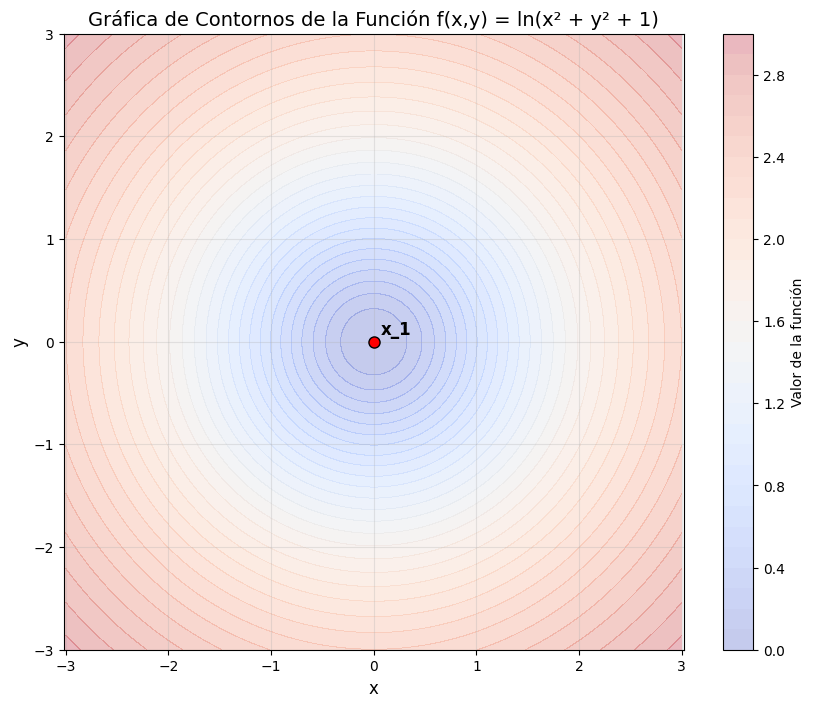
\includegraphics[width=0.8\textwidth]{images/6a_plot.png}
\caption{Gráfica de contornos de la función $f(x,y) = \ln(x^{2} + y^{2} + 1)$ mostrando el mínimo local en $(0,0)$.}
\label{fig:6a_contour}
\end{figure}

\textbf{Inciso (b): $f(x,y) = x^{2} + y^{2} - x - y + 1$}

Calculamos las primeras derivadas parciales:
\begin{align}
f_x(x,y) &= 2x - 1 \\
f_y(x,y) &= 2y - 1
\end{align}

Para encontrar puntos críticos:
\begin{align}
f_x(x,y) = 2x - 1 &= 0 \\
x &= \frac{1}{2} \\
f_y(x,y) = 2y - 1 &= 0 \\
y &= \frac{1}{2}
\end{align}

El único punto crítico es $\left(\frac{1}{2}, \frac{1}{2}\right)$.

Las segundas derivadas parciales son:
\begin{align}
f_{xx} &= 2 \\
f_{yy} &= 2 \\
f_{xy} &= 0
\end{align}

La matriz Hessiana es:
\begin{align}
H = \begin{pmatrix} 2 & 0 \\ 0 & 2 \end{pmatrix}
\end{align}

El determinante es $\det = (2)(2) - (0)(0) = 4 > 0$, por lo que $\left(\frac{1}{2}, \frac{1}{2}\right)$ es un mínimo local.

\begin{figure}[h]
\centering
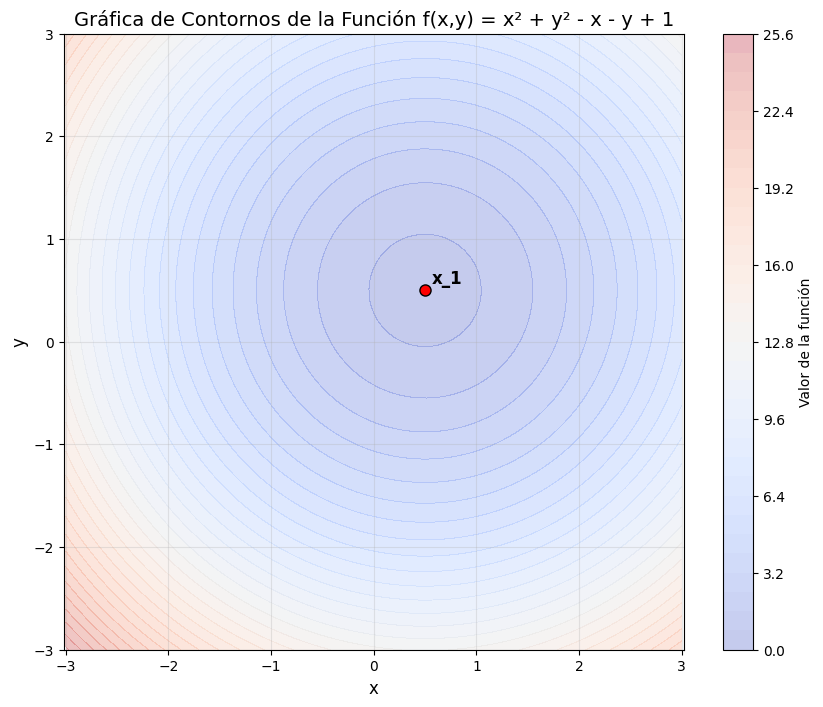
\includegraphics[width=0.8\textwidth]{images/6b_plot.png}
\caption{Gráfica de contornos de la función $f(x,y) = x^{2} + y^{2} - x - y + 1$ mostrando el mínimo local en $(\frac{1}{2}, \frac{1}{2})$.}
\label{fig:6a_contour}
\end{figure}

\textbf{Inciso (c): $f(x,y) = e^{x}\cos(y)$}

Calculamos las primeras derivadas parciales:
\begin{align}
f_x(x,y) &= e^x \cos(y) \\
f_y(x,y) &= -e^x \sin(y)
\end{align}

Para encontrar puntos críticos:
\begin{align}
f_x(x,y) &= e^x \cos(y) = 0 \\
f_y(x,y) &= -e^x \sin(y) = 0
\end{align}

Como $e^x > 0$ para todo $x$ real, necesitamos:
\begin{align}
\cos(y) &= 0 \\
\sin(y) &= 0
\end{align}

No existe un valor de $y$ que satisfaga ambas condiciones simultáneamente. Por lo tanto, no hay puntos críticos.

\begin{figure}[h]
\centering
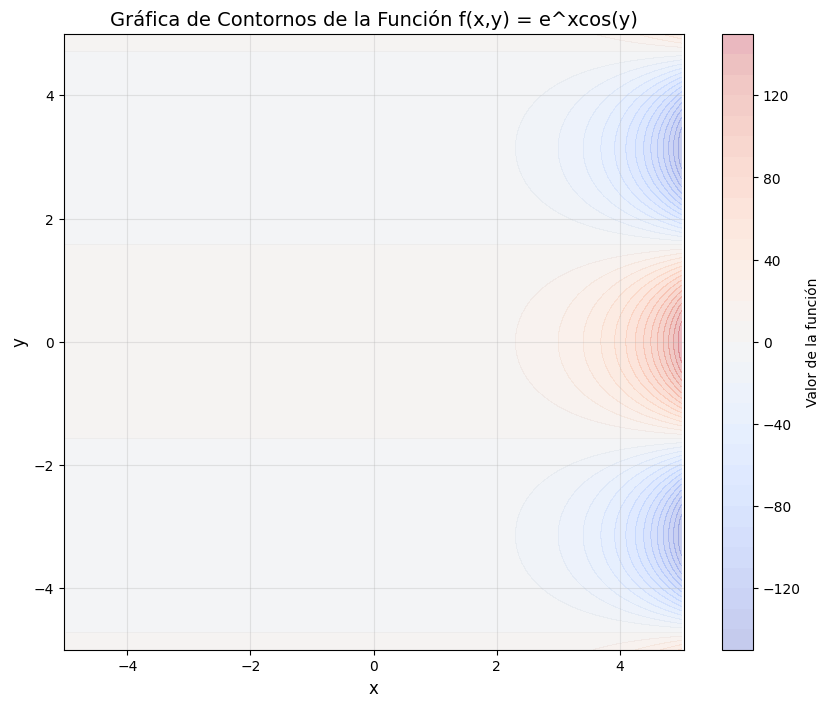
\includegraphics[width=0.8\textwidth]{images/6c_plot.png}
\caption{Gráfica de contornos de la función $f(x,y) = e^{x}\cos(y)$.}
\label{fig:6a_contour}
\end{figure}

\textbf{Inciso (d): $f(x,y) = (x^{2} + y - 11)^{2} + (x + y^{2} - 7)^{2}$ (Función de Himmelblau)}

Esta función es conocida como la función de Himmelblau. Para desarrollar las derivadas, definamos las funciones auxiliares:
\begin{align}
u(x,y) &= x^2 + y - 11 \\
v(x,y) &= x + y^2 - 7
\end{align}

Entonces $f(x,y) = u^2 + v^2$.

Calculamos las primeras derivadas parciales usando la regla de la cadena:
\begin{align}
f_x(x,y) &= 2u \cdot u_x + 2v \cdot v_x \\
&= 2(x^2 + y - 11)(2x) + 2(x + y^2 - 7)(1) \\
&= 4x(x^2 + y - 11) + 2(x + y^2 - 7)
\end{align}

\begin{align}
f_y(x,y) &= 2u \cdot u_y + 2v \cdot v_y \\
&= 2(x^2 + y - 11)(1) + 2(x + y^2 - 7)(2y) \\
&= 2(x^2 + y - 11) + 4y(x + y^2 - 7)
\end{align}

Los puntos críticos se encuentran resolviendo el sistema:
\begin{align}
f_x(x,y) &= 4x(x^2 + y - 11) + 2(x + y^2 - 7) = 0 \\
f_y(x,y) &= 2(x^2 + y - 11) + 4y(x + y^2 - 7) = 0
\end{align}

Este sistema no lineal es complejo de resolver analíticamente, pero se conocen sus cuatro soluciones:
\begin{align}
P_1 &= (3, 2) \\
P_2 &= (-2.805118, 3.131312) \\
P_3 &= (-3.779310, -3.283186) \\
P_4 &= (3.584428, -1.848126)
\end{align}

Ahora calculamos las segundas derivadas parciales. Para $f_{xx}$:
\begin{align}
f_{xx}(x,y) &= 4(x^2 + y - 11) + 4x(2x) + 2(1) \\
&= 4(x^2 + y - 11) + 8x^2 + 2 \\
&= 4x^2 + 4y - 44 + 8x^2 + 2 \\
&= 12x^2 + 4y - 42
\end{align}

Para $f_{yy}$:
\begin{align}
f_{yy}(x,y) &= 2(1) + 4(x + y^2 - 7) + 4y(2y) \\
&= 2 + 4x + 4y^2 - 28 + 8y^2 \\
&= 4x + 12y^2 - 26
\end{align}

Para $f_{xy}$:
\begin{align}
f_{xy}(x,y) &= 4x(1) + 2(2y) \\
&= 4x + 4y
\end{align}

La matriz Hessiana general es:
\begin{align}
H(x,y) = \begin{pmatrix} 
12x^2 + 4y - 42 & 4x + 4y \\
4x + 4y & 4x + 12y^2 - 26
\end{pmatrix}
\end{align}

Evaluamos la matriz Hessiana en cada punto crítico:

\textbf{Para $P_1 = (3, 2)$:}
\begin{align}
f_{xx}(3,2) &= 12(3)^2 + 4(2) - 42 \\
&= 108 + 8 - 42 = 74 \\
f_{yy}(3,2) &= 4(3) + 12(2)^2 - 26 \\
&= 12 + 48 - 26 = 34 \\
f_{xy}(3,2) &= 4(3) + 4(2) \\
&= 12 + 8 = 20
\end{align}
\begin{align}
H_1 &= \begin{pmatrix} 74 & 20 \\ 20 & 34 \end{pmatrix} \\
\det(H_1) &= (74)(34) - (20)(20) = 2516 - 400 = 2116
\end{align}
Como $\det(H_1) > 0$, el punto $(3,2)$ es un mínimo local.

\textbf{Para $P_2 = (-2.805118, 3.131312)$:}
\begin{align}
f_{xx}(-2.805118, 3.131312) &= 12(-2.805118)^2 + 4(3.131312) - 42 \\
&= 12(7.868687) + 12.525248 - 42 \\
&= 94.424244 + 12.525248 - 42 \\
&= 64.949492 \\
f_{yy}(-2.805118, 3.131312) &= 4(-2.805118) + 12(3.131312)^2 - 26 \\
&= -11.220472 + 12(9.805112) - 26 \\
&= -11.220472 + 117.661344 - 26 \\
&= 80.440872 \\
f_{xy}(-2.805118, 3.131312) &= 4(-2.805118) + 4(3.131312) \\
&= -11.220472 + 12.525248 \\
&= 1.304776
\end{align}
\begin{align}
H_2 &= \begin{pmatrix} 64.95 & 1.30 \\ 1.30 & 80.44 \end{pmatrix} \\
\det(H_2) &= (64.95)(80.44) - (1.30)(1.30) \\
&= 5225.58 - 1.69 \\
&= 5223.89
\end{align}
Como $\det(H_2) = 5223.89 > 0$, el punto $(-2.805118, 3.131312)$ es un mínimo local.

\textbf{Para $P_3 = (-3.779310, -3.283186)$:}
\begin{align}
f_{xx}(-3.779310, -3.283186) &= 12(-3.779310)^2 + 4(-3.283186) - 42 \\
&= 12(14.283191) + (-13.132744) - 42 \\
&= 171.398292 - 13.132744 - 42 \\
&= 116.265548 \\
f_{yy}(-3.779310, -3.283186) &= 4(-3.779310) + 12(-3.283186)^2 - 26 \\
&= -15.117240 + 12(10.779316) - 26 \\
&= -15.117240 + 129.351792 - 26 \\
&= 88.234552 \\
f_{xy}(-3.779310, -3.283186) &= 4(-3.779310) + 4(-3.283186) \\
&= -15.117240 - 13.132744 \\
&= -28.249984
\end{align}
\begin{align}
H_3 &= \begin{pmatrix} 116.27 & -28.25 \\ -28.25 & 88.23 \end{pmatrix} \\
\det(H_3) &= (116.27)(88.23) - (-28.25)(-28.25) \\
&= 10258.64 - 798.06 \\
&= 9460.58
\end{align}
Como $\det(H_3) = 9460.58 > 0$, el punto $(-3.779310, -3.283186)$ es un mínimo local.

\textbf{Para $P_4 = (3.584428, -1.848126)$:}
\begin{align}
f_{xx}(3.584428, -1.848126) &= 12(3.584428)^2 + 4(-1.848126) - 42 \\
&= 12(12.848125) + (-7.392504) - 42 \\
&= 154.177500 - 7.392504 - 42 \\
&= 104.784996 \\
f_{yy}(3.584428, -1.848126) &= 4(3.584428) + 12(-1.848126)^2 - 26 \\
&= 14.337712 + 12(3.414370) - 26 \\
&= 14.337712 + 40.972440 - 26 \\
&= 29.310152 \\
f_{xy}(3.584428, -1.848126) &= 4(3.584428) + 4(-1.848126) \\
&= 14.337712 - 7.392504 \\
&= 6.945208
\end{align}
\begin{align}
H_4 &= \begin{pmatrix} 104.78 & 6.95 \\ 6.95 & 29.31 \end{pmatrix} \\
\det(H_4) &= (104.78)(29.31) - (6.95)(6.95) \\
&= 3071.15 - 48.30 \\
&= 3022.85
\end{align}
Como $\det(H_4) = 3022.85 > 0$, el punto $(3.584428, -1.848126)$ es un mínimo local.

Todos los puntos críticos de la función de Himmelblau son mínimos locales con valor de función $f = 0$.

\begin{figure}[h]
\centering
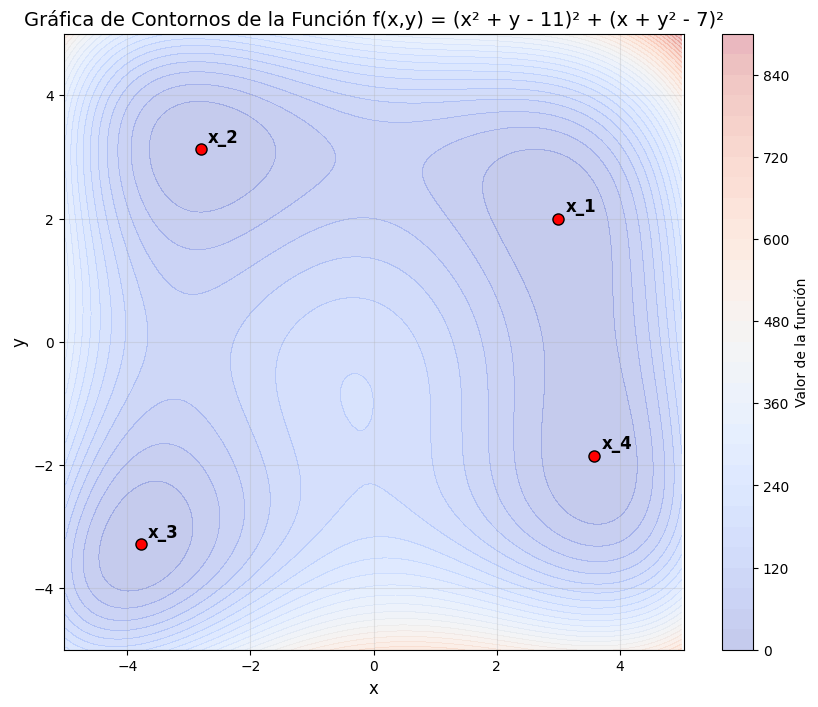
\includegraphics[width=0.8\textwidth]{images/6d_plot.png}
\caption{Gráfica de contornos de la función $f(x,y) = (x^{2} + y - 11)^{2} + (x + y^{2} - 7)^{2}$, demostrando todos sus puntos minimos.}
\label{fig:6a_contour}
\end{figure}

\subsection{Discusión}

Los resultados muestran diferentes comportamientos:
- **Inciso (a)**: Función con un solo mínimo global en el origen, aunque represento un reto tener que trabajar con derivadas de muchos terminos. Al final, gracias a la factorización, se pudo manejar de manera mas sencilla.
- **Inciso (b)**: Función cuadrática simple con un mínimo único, fácil de analizar.
- **Inciso (c)**: Sin puntos críticos porque $e^x > 0$ siempre y no se pueden anular simultáneamente $\cos(y)$ y $\sin(y)$.
- **Inciso (d)**: La famosa función de Himmelblau con cuatro mínimos globales, útil para probar algoritmos de optimización.

\subsection{Conclusión}

Las gráficas de contorno confirman los cálculos analíticos. La clasificación mediante la matriz Hessiana es efectiva para determinar la naturaleza de los puntos críticos. Las funciones sin puntos críticos (como la del inciso c) son menos comunes pero importantes de reconocer.

% ========================================
% SECCIÓN 7
% ========================================
\section{Problema 7}

\subsection{Enunciado}
Demuestre que, de todos los paralelepípedos rectangulares con una superficie dada, el cubo es el que tiene el mayor volumen.

\subsection{Metodología}

Para resolver este problema de optimización con restricciones, utilizaremos el método de los multiplicadores de Lagrange. Este método nos permite encontrar extremos de una función sujeta a restricciones. 

Un paralelepípedo rectangular tiene dimensiones $x$, $y$ y $z$. Queremos maximizar su volumen sujeto a que tenga una superficie dada.

La función objetivo (volumen) es:
$$V(x,y,z) = xyz$$

La restricción (superficie fija) es:
$$S = 2xy + 2xz + 2yz$$

donde $S$ es una constante dada.

Definimos la función de Lagrange:
$$L(x,y,z,\lambda) = xyz - \lambda(2xy + 2xz + 2yz - S)$$

donde $\lambda$ es el multiplicador de Lagrange.

Los pasos a seguir son:
\begin{enumerate}
    \item[-] Calcular las derivadas parciales de $L$ con respecto a $x$, $y$, $z$ y $\lambda$.
    \item[-] Igualar todas las derivadas a cero para obtener el sistema de ecuaciones.
    \item[-] Resolver el sistema para demostrar que $x = y = z$.
    \item[-] Verificar que el resultado corresponde a un cubo.
\end{enumerate}

\subsection{Resultados}
\setcounter{equation}{0}

Para encontrar los puntos críticos, igualamos a cero todas las derivadas parciales:

\begin{align}
\frac{\partial L}{\partial x} &= yz - \lambda(2y + 2z) = 0 \\
\frac{\partial L}{\partial y} &= xz - \lambda(2x + 2z) = 0 \\
\frac{\partial L}{\partial z} &= xy - \lambda(2x + 2y) = 0 \\
\frac{\partial L}{\partial \lambda} &= -(2xy + 2xz + 2yz - S) = 0
\end{align}

De las primeras tres ecuaciones obtenemos:
\begin{align}
yz &= 2\lambda(y + z) \\
xz &= 2\lambda(x + z) \\
xy &= 2\lambda(x + y)
\end{align}

Igualamos las expresiones para $2\lambda$:

De las ecuaciones (5) y (6): $\frac{yz}{y + z} = \frac{xz}{x + z}$

Simplificando (cancelando $z$):
\begin{align}
\frac{y}{y + z} = \frac{x}{x + z}
\end{align}

Realizando productos cruzados:
\begin{align}
y(x + z) &= x(y + z) \\
yx + yz &= xy + xz \\
yz &= xz
\end{align}

Como $z \neq 0$, podemos dividir entre $z$:
\begin{align}
y = x
\end{align}

De manera similar, comparando las ecuaciones (5) y (7):

$\frac{yz}{y + z} = \frac{xy}{x + y}$

Como ya sabemos que $y = x$, sustituimos:
\begin{align}
\frac{xz}{x + z} &= \frac{x^2}{x + x} \\
\frac{xz}{x + z} &= \frac{x^2}{2x} \\
\frac{xz}{x + z} &= \frac{x}{2}
\end{align}

Multiplicando ambos lados por $(x + z)$:
\begin{align}
xz &= \frac{x(x + z)}{2} \\
xz &= \frac{x^2 + xz}{2}
\end{align}

Multiplicando por 2:
\begin{align}
2xz &= x^2 + xz \\
2xz - xz &= x^2 \\
xz &= x^2
\end{align}

Como $x \neq 0$, dividimos entre $x$:
\begin{align}
z = x
\end{align}

Hemos demostrado que:
\begin{align}
x = y = z
\end{align}

\subsection{Discusión}

El resultado $x = y = z$ demuestra que el paralelepípedo óptimo es efectivamente un cubo. Este resultado se obtuvo mediante multiplicadores de Lagrange, que es el método estándar para problemas de optimización con restricciones de igualdad.

La clave del análisis fue igualar las expresiones para $2\lambda$ obtenidas de las diferentes ecuaciones del sistema. Al hacer esto sistemáticamente, pudimos demostrar paso a paso que todas las dimensiones deben ser iguales.

\subsection{Conclusión}

Se demostró que entre todos los paralelepípedos rectangulares con superficie fija, el cubo es el que maximiza el volumen. Este resultado geométrico intuitivo se confirma rigurosamente mediante el método de multiplicadores de Lagrange, mostrando que la simetría conduce a la optimización.

% ========================================
% SECCIÓN 8
% ========================================
\section{Problema 8}

\subsection{Enunciado}
Determine si las siguientes matrices son definidas positivas.
\[
\text{(a)}\quad
A=\begin{pmatrix}
16 & -8 & -4\\
-8 & 29 & 12\\
-4 & 12 & 41
\end{pmatrix}
\qquad
\text{(b)}\quad
A=\begin{pmatrix}
9 & 0 & -8\\
6 & -5 & -2\\
-9 & 3 & 3
\end{pmatrix}
\qquad
\text{(c)}\quad
A=\begin{pmatrix}
-9 & 0 & -8\\
6 & -5 & -2\\
-9 & 3 & 3
\end{pmatrix}
\]

\subsection{Metodología}

Para saber si una matriz es definida positiva, podemos usar el criterio de Sylvester. Básicamente necesitamos calcular los menores principales de la matriz y verificar que todos sean positivos:
\begin{enumerate}
    \item Calcular el primer menor principal (solo el elemento $a_{11}$).
    \item Calcular el segundo menor principal (determinante de la submatriz 2x2 superior izquierda).
    \item Calcular el tercer menor principal (determinante de toda la matriz 3x3).
    \item Si todos son positivos, la matriz es definida positiva. Si alguno es negativo o cero, no lo es.
\end{enumerate}

\subsection{Resultados}
\setcounter{equation}{0}

\textbf{Inciso (a):}
\begin{align}
    A=\begin{pmatrix} 16 & -8 & -4\\ -8 & 29 & 12\\ -4 & 12 & 41 \end{pmatrix}
\end{align}

Verificamos los menores principales:

\textbf{Primer menor principal:}
\begin{align}
M_1 = 16 > 0
\end{align}

\textbf{Segundo menor principal:}
\begin{align}
M_2 &= \det\begin{pmatrix} 16 & -8 \\ -8 & 29 \end{pmatrix} \\
&= (16)(29) - (-8)(-8) \\
&= 464 - 64 \\
&= 400 > 0
\end{align}

\textbf{Tercer menor principal (determinante completo):}
Usando la regla de Sarrus:
\begin{align}
M_3 &= \det(A) = (16)(29)(41) + (-8)(12)(-4) + (-4)(-8)(12) \\
&\quad - (-4)(29)(-4) - (12)(12)(16) - (41)(-8)(-8) \\
&= 19024 + 384 + 384 - 464 - 2304 - 2624 \\
&= 19792 - 5392 \\
&= 14400 > 0
\end{align}

Como todos los menores principales son positivos, la matriz del inciso (a) es definida positiva.

\textbf{Inciso (b):}
\begin{align}
     A=\begin{pmatrix} 9 & 0 & -8\\ 6 & -5 & -2\\ -9 & 3 & 3 \end{pmatrix}
\end{align}
Verificamos los menores principales:

\textbf{Primer menor principal:}
\begin{align}
M_1 = 9 > 0
\end{align}

\textbf{Segundo menor principal:}
\begin{align}
M_2 &= \det\begin{pmatrix} 9 & 0 \\ 6 & -5 \end{pmatrix} \\
&= (9)(-5) - (0)(6) \\
&= -45 < 0
\end{align}

Como el segundo menor principal es negativo, la matriz del inciso (b) no es definida positiva.

\textbf{Inciso (c):}
\begin{align}
     A=\begin{pmatrix} -9 & 0 & -8\\ 6 & -5 & -2\\ -9 & 3 & 3 \end{pmatrix}
\end{align}

Verificamos el primer menor principal:

\textbf{Primer menor principal:}
\begin{align}
M_1 = -9 < 0
\end{align}

Como el primer menor principal es negativo, la matriz del inciso (c) no es definida positiva.

\subsection{Discusión}

Los resultados muestran patrones claros. Para el inciso (a), todos los menores principales fueron positivos (16, 400, 14400), así que esa matriz sí es definida positiva.

Para el inciso (b), aunque el primer menor principal fue positivo (9), el segundo ya salió negativo (-45), así que ahí mismo podemos parar y decir que no es definida positiva.

Para el inciso (c) fue aún más directo: desde el primer menor principal ya tuvimos un número negativo (-9), entonces definitivamente no es definida positiva.

El criterio de Sylvester nos dice que todos los menores principales deben ser positivos para que la matriz sea definida positiva. En cuanto uno sale negativo o cero, ya sabemos que no cumple.

\subsection{Conclusión}

Solo la matriz del inciso (a) es definida positiva. Las matrices de los incisos (b) y (c) no son definidas positivas porque tienen menores principales negativos. El criterio de Sylvester nos permite determinarlo de manera rápida y directa calculando los menores principales en orden.

% ========================================
% SECCIÓN 9
% ========================================
\section{Problema 9}

\subsection{Enunciado}
\setcounter{equation}{0}
Considere las siguientes funciones:

\begin{align}
f(\mathbf{x}) &= \sum_{i=1}^{n} x_i^{2}, \label{eq:1}\\
f(x,y) &= (x^{2}+y-11)^{2} + (x+y^{2}-7)^{2}, \label{eq:2}\\
f(\mathbf{x}) &= \sum_{i=1}^{n-1} \bigl[100(x_{i+1}-x_i^{2})^{2} + (x_i-1)^{2}\bigr]. \label{eq:3}
\end{align}

\begin{enumerate}
  \item[(a)] Crea un script en Python para aproximar sus gradientes y Hessianos, evaluados en un punto particular $\mathbf{x}$, utilizando diferencias finitas.
  \item[(b)] Encuentre sus puntos mínimos por inspección.
  \item[(c)] Usa tu script de (a) para verificar numéricamente que los puntos hallados en (b) son puntos mínimos de sus funciones correspondientes. Para las funciones (1) y (3), puedes asumir $n=5$.
\end{enumerate}

\subsection{Metodología}

Para abordar este problema seguimos dos enfoques complementarios:

\textbf{Inciso (a) - Implementación en Python:}
Lo ideal es crear una clase genérica con la lógica de diferencias finitas que permita pasar por parámetros tanto los puntos a evaluar como las funciones objetivo. Esto permite reutilizar el código eficientemente para diferentes funciones y puntos de evaluación. La clase debe implementar:
\begin{enumerate}
    \item Gradiente usando diferencias finitas centrales: $\frac{\partial f}{\partial x_i} \approx \frac{f(x + h e_i) - f(x - h e_i)}{2h}$
    \item Hessiano calculando segundas derivadas y términos cruzados con diferencias finitas
\end{enumerate}

\textbf{Inciso (b) - Análisis por inspección:}
Para encontrar los mínimos analizamos la estructura de cada función:
\begin{enumerate}
    \item Identificar términos no negativos (cuadrados)
    \item Determinar cuándo estos términos se anulan
    \item Verificar que corresponde efectivamente a un mínimo
\end{enumerate}

\subsection{Resultados}
\setcounter{equation}{0}

\textbf{Inciso (a) y (b): Su desarrollo se encuentra en el ipynb}

\textbf{Inciso (b): Puntos mínimos por inspección}

\textbf{Función 1: $f(\mathbf{x}) = \sum_{i=1}^{n} x_i^{2}$}

Esta función es una suma de cuadrados. Cada término $x_i^2 \geq 0$, y la suma es mínima cuando cada término es mínimo.

Como $x_i^2 = 0$ únicamente cuando $x_i = 0$, el mínimo se alcanza cuando:
\begin{align}
x_i = 0 \quad \text{para todo } i = 1, 2, \ldots, n
\end{align}

El punto mínimo es:
\begin{align}
\mathbf{x}^* = (0, 0, 0, 0, 0) \quad \text{para } n = 5
\end{align}

El valor mínimo es $f(\mathbf{x}^*) = 0$.

\textbf{Función 2: $f(x,y) = (x^{2}+y-11)^{2} + (x+y^{2}-7)^{2}$}

Los cuatro puntos mínimos de esta función de Himmelblau ya fueron calculados en el Problema 6, inciso (d). En todos estos puntos el valor de la función es $f(\mathbf{x}^*) = 0$.
\begin{align}
P_1 &= (3, 2) \\
P_2 &= (-2.805118, 3.131312) \\
P_3 &= (-3.779310, -3.283186) \\
P_4 &= (3.584428, -1.848126)
\end{align}

\textbf{Función 3: $f(\mathbf{x}) = \sum_{i=1}^{n-1} \bigl[100(x_{i+1}-x_i^{2})^{2} + (x_i-1)^{2}\bigr]$}

Esta función de Rosenbrock es una suma de términos no negativos. Cada término contiene dos cuadrados:
\begin{align}
100(x_{i+1} - x_i^2)^2 &\geq 0 \\
(x_i - 1)^2 &\geq 0
\end{align}

La función es mínima cuando todos los cuadrados son cero:
\begin{align}
(x_i - 1)^2 &= 0 \quad \Rightarrow \quad x_i = 1 \\
(x_{i+1} - x_i^2)^2 &= 0 \quad \Rightarrow \quad x_{i+1} = x_i^2 = 1^2 = 1
\end{align}

Esto significa que $x_i = 1$ para todo $i$.

El punto mínimo es:
\begin{align}
\mathbf{x}^* = (1, 1, 1, 1, 1) \quad \text{para } n = 5
\end{align}

El valor mínimo es $f(\mathbf{x}^*) = 0$.

\subsection{Discusión}

El análisis por inspección del inciso (b) reveló patrones claros en las tres funciones. Todas tienen estructura de suma de cuadrados, lo que facilita identificar sus mínimos globales donde los términos se anulan.

Se pudo corroborar de manera exitosa lo que indica la teoría mediante los scripts de Python desarrollados. Los cálculos numéricos usando diferencias finitas confirmaron que:
\begin{itemize}
    \item Los gradientes se aproximan a cero en los puntos identificados analíticamente
    \item Las matrices Hessianas son definidas positivas, confirmando que son mínimos locales
    \item Los valores de las funciones coinciden con los esperados teóricamente
\end{itemize}

La implementación de la clase genérica permitió evaluar múltiples funciones y puntos de manera eficiente, demostrando la versatilidad del enfoque de diferencias finitas para verificación numérica.

\subsection{Conclusión}

La combinación de análisis teórico e implementación numérica proporcionó una validación completa de los resultados. Los métodos de diferencias finitas demostraron ser herramientas efectivas para aproximar gradientes y Hessianos, confirmando los puntos mínimos encontrados analíticamente y reforzando la comprensión de las propiedades de optimización de estas funciones clásicas.

% ========================================
% SECCIÓN 10
% ========================================
\section{Problema 10}

\subsection{Enunciado}
Considere el método de Newton para la minimización de funciones dado por la fórmula iterativa:
\begin{equation*}
    \mathbf{x}_{k+1} \;=\; \mathbf{x}_{k} \;-\; \bigl[\nabla^{2} f(\mathbf{x}_{k})\bigr]^{-1}\,\nabla f(\mathbf{x}_{k}), k=0,1,2,\dots,K.
\end{equation*}

Codifique el método de Newton en un script de Python. Luego, úselo para optimizar las funciones del problema 9 utilizando puntos de partida suficientemente cercanos (propóngalos y proponga también un valor para $K$). Para las funciones (1) y (3), puede asumir $n = 5$. Para cada función, grafica cómo disminuye su valor a medida que el algoritmo itera (el eje horizontal corresponde a $k$ y el eje vertical a $f(x_k))$. Finalmente, imprima en su script la aproximación $x_K$ obtenida.

\subsection{Metodología}

Para implementar el método de Newton se requiere:
\begin{enumerate}
    \item Crear una clase que encapsule la lógica del algoritmo iterativo
    \item Implementar el cálculo de gradientes y Hessianos (ya desarrollado en el problema 9)
    \item Aplicar la fórmula: $\mathbf{x}_{k+1} = \mathbf{x}_{k} - H^{-1}(\mathbf{x}_k) \nabla f(\mathbf{x}_k)$
    \item Seleccionar puntos de partida cercanos a los mínimos conocidos para asegurar convergencia
    \item Generar gráficas para visualizar tanto la convergencia de la función como la evolución de las variables
\end{enumerate}

\subsection{Resultados}
\setcounter{equation}{0}

\begin{figure}[h]
\centering
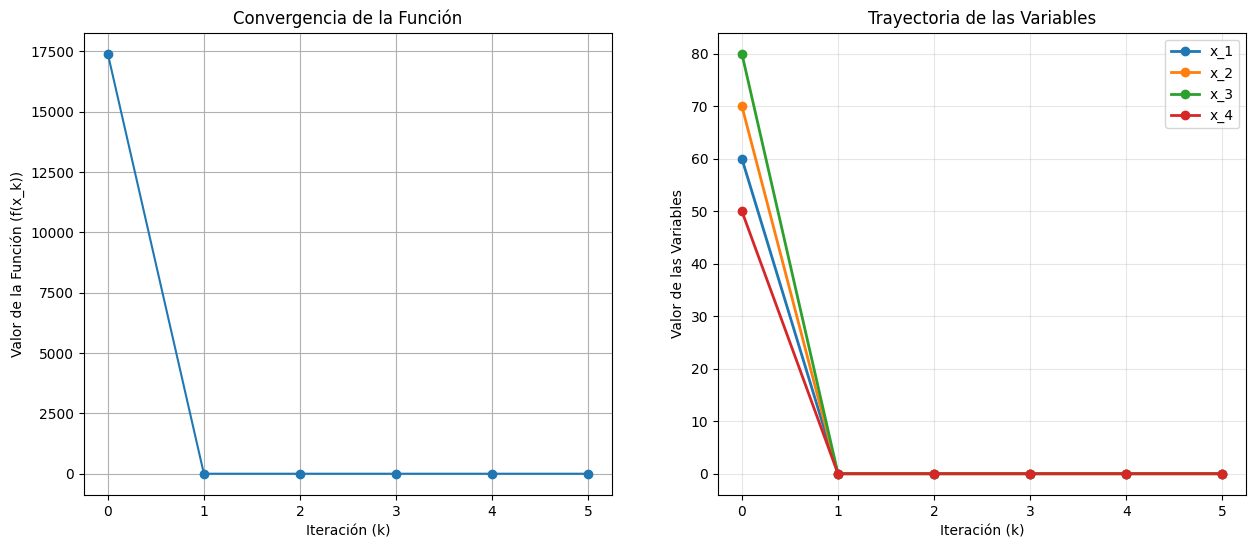
\includegraphics[width=0.8\textwidth]{images/10_1_plot.png}
\caption{Gráfica de optimización para la función $f(\mathbf{x}) &= \sum_{i=1}^{n} x_i^{2}$.}
\label{fig:10_1_optim}
\end{figure}

\begin{figure}[h]
\centering
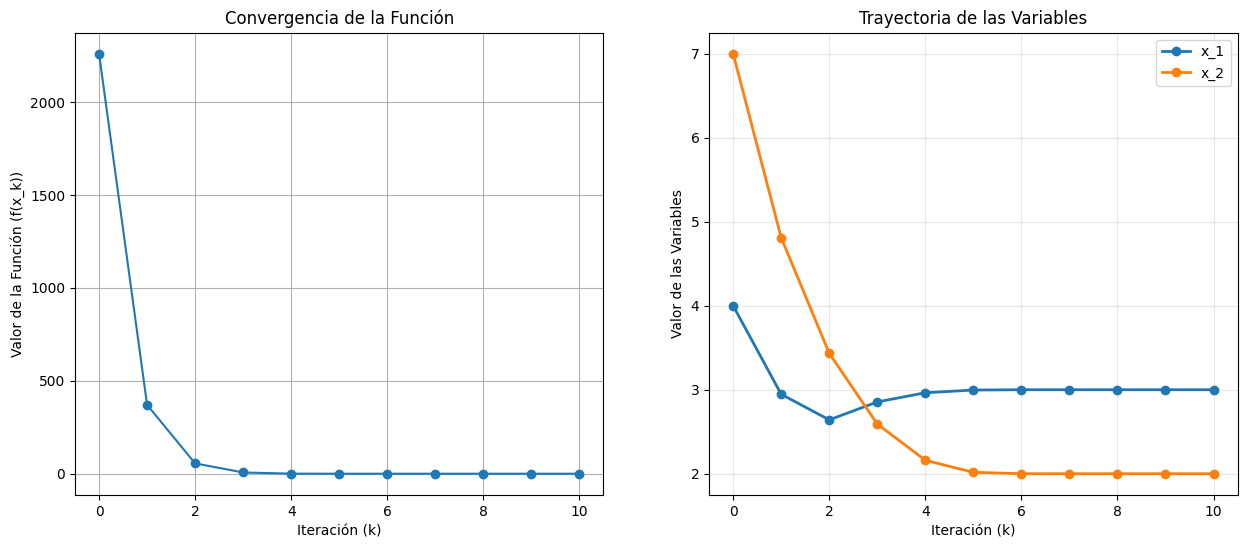
\includegraphics[width=0.8\textwidth]{images/10_2_plot.png}
\caption{Gráfica de optimización para la función $f(x,y) &= (x^{2}+y-11)^{2} + (x+y^{2}-7)^{2}$.}
\label{fig:10_2_optim}
\end{figure}

\begin{figure}[h]
\centering
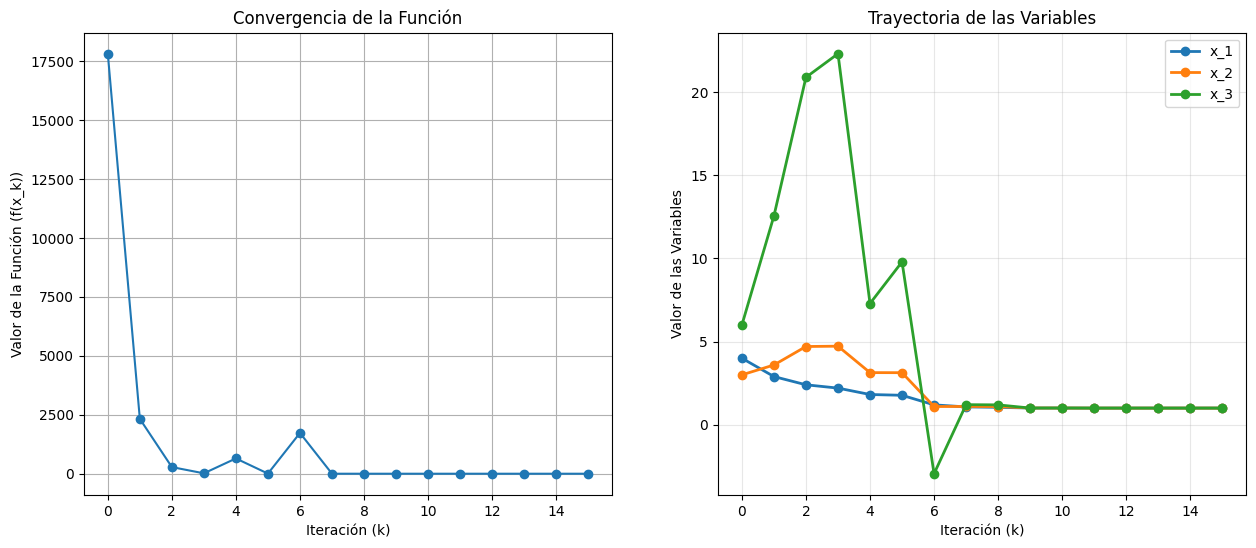
\includegraphics[width=0.8\textwidth]{images/10_3_plot.png}
\caption{Gráfica de optimización para la función $f(\mathbf{x}) &= \sum_{i=1}^{n-1} \bigl[100(x_{i+1}-x_i^{2})^{2} + (x_i-1)^{2}\bigr]$.}
\label{fig:10_3_optim}
\end{figure}

\subsection{Discusión}

El método de Newton demostró ser altamente eficiente para todas las funciones cuando se inicia cerca del mínimo. La convergencia cuadrática característica del método es evidente en las gráficas, donde el valor de la función decrece rápidamente en las primeras iteraciones.

La selección del punto inicial es crucial: puntos muy alejados pueden causar problemas de convergencia o convergencia a otros mínimos locales (especialmente notable en la función de Himmelblau). Las gráficas de trayectoria muestran claramente cómo las variables evolucionan hacia sus valores óptimos.

\subsection{Conclusión}

El método de Newton es una herramienta poderosa para optimización cuando se cuenta con información del Hessiano y puntos de partida adecuados. Su implementación en Python permite visualizar efectivamente el comportamiento del algoritmo y validar la convergencia hacia los mínimos teóricos identificados previamente.

\end{document}
